\section{Results}

\subsection{Benchmark of values}

\begin{itemize}

  \item \textbf{Image: gain VS time for one single point. Overlay between
    experiment/daniels sim/our sim}

  \item comparison with previous values from Daniel's thesis

  \item (comparison with results from an experiment)

\end{itemize}



\subsection{runtimes}

\begin{itemize}

  \item \textbf{Image: Comparison between for\_loops, fixed and adaptive
    numberOfRays for a single wavelength} (use a reasonable MSE)
    \begin{figure}[H]
      \centerline{
        \resizebox{0.45\textwidth}{!}{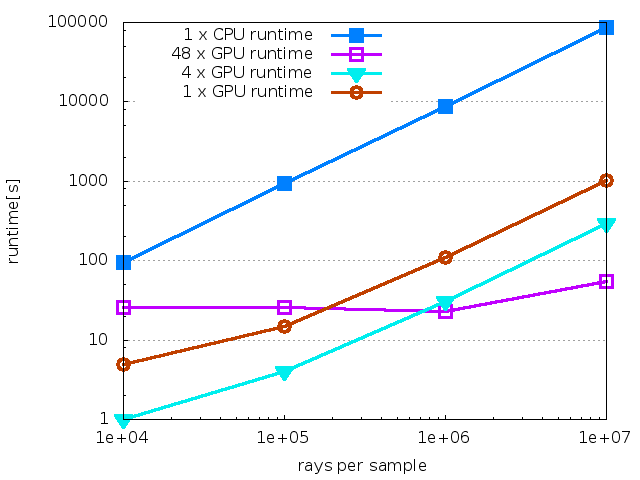
\includegraphics[width=8cm]{plot/runtime.png}}}
      \caption{Comparision implementation}
      \label{plot:runtime}
    \end{figure}

  \item good speedup through parallelization

  \item adaptive number of rays MUCH faster than fixed number of rays

  \item \textbf{Image: runtime VS precision of simulation} (precision based on
    MSE)

  \item use MSE to adjust the precision of the simulation rather than
    increasing the default number of rays

  \item law of diminishing returns: to lower the MSE below a certain threshold,
    exponentially more rays are required

  \item very low computation times result in values comparable to extremly long
    simulations.

  \item \textbf{Image: MultiGPU with different number of devices VS time}

  \item distributing the computation to multiple devices scales well

\end{itemize}
